\section{Results}
\label{sec:results}

\subsection{What goes wrong physically}
\label{sec:physics}

\begin{table}[t]
\centering
\caption{Physics of the generated motions (range over seeds; 1,000 motions per seed). Jump gravity is the median fitted fall rate of unsupported airborne stretches that do fall (real flight: 9.81\,m/s$^2$); floating counts unsupported stretches that barely fall. Here ``jump prompts'' are the 14 curated jump prompts of the main runs (Section~\ref{sec:models}); elsewhere the term means the jump-heavy runs.}
\label{tab:physics}
\begin{tabular}{lcc}
\toprule
Measure & 50-step (3 seeds) & 1000-step (3 seeds) \\
\midrule
Floating, \% of frames, jump prompts & 0.6--0.8 & 4.8--9.3 \\
Floating, \% of frames, test captions & 3.8--4.7 & 8.6--9.7 \\
Jump gravity, median (m/s$^2$), jump prompts & 9.54--9.75 & 9.13--9.22 \\
Jump gravity, median (m/s$^2$), test captions & 9.07--9.84 & 8.59--9.78 \\
Raised contact ($>$5\,cm), \% of contact frames, jump prompts & 1.2--2.4 & 3.0--8.4 \\
Raised contact ($>$5\,cm), \% of contact frames, test captions & 2.9--3.3 & 4.9--5.4 \\
\bottomrule
\end{tabular}

\end{table}

When MDM's bodies leave the ground and fall, they fall at close to the right rate (Table~\ref{tab:physics}): the median fitted gravity on the curated jump prompts is 9.54 to 9.75\,m/s$^2$ for the 50-step model and 9.13 to 9.22\,m/s$^2$ for the 1000-step model, somewhat slower than real jumps in the processed form of its training data (median 10.33\,m/s$^2$, Appendix~\ref{app:realmotion}). Individual stretches spread widely around these medians (standard deviation 2.24\,m/s$^2$ on the jump-heavy runs, against 0.7 to 1.0\,m/s$^2$ for real jumps). The common failure is floating. On HumanML3D test captions, 3.8 to 4.7\% of the 50-step model's frames lie in floating stretches, against 8.6 to 9.7\% for the 1000-step model. On the curated jump prompts the figures are 0.6 to 0.8\% and 4.8 to 9.3\%. The raised-contact rate, a foot in contact but more than 5\,cm up, follows the same pattern. Part of the floating is implied by the prompt: a person ``walking on a balance beam'' is generated without a beam and floats in nearly every sample. On test captions the original 1000-step checkpoint floats about twice as often as the 50-step one, in all three seeds and under every threshold setting we tried (Appendix~\ref{app:sensitivity}). On real motion capture the same labels flag floating in 0.09\% of frames (Appendix~\ref{app:realmotion}).

A typical floating stretch is an ordinary walking pose with the whole body several centimeters off the floor for about half a second, in a motion that touches the floor elsewhere (Figure~\ref{fig:teaser}, Appendix~\ref{app:labelfix}). Our first definition of airborne looked only at the feet, so it fitted such stretches, and stretches supported by the hands or knees, as flight. That made the 1000-step model's jumps appear to fall far too slowly (medians of 3.75 and 7.55\,m/s$^2$ in the two seeds labelled that way), an effect that disappears once floating is separated out.

\subsection{Physics is readable early in denoising}
\label{sec:readable}

\begin{figure}[t]
\centering
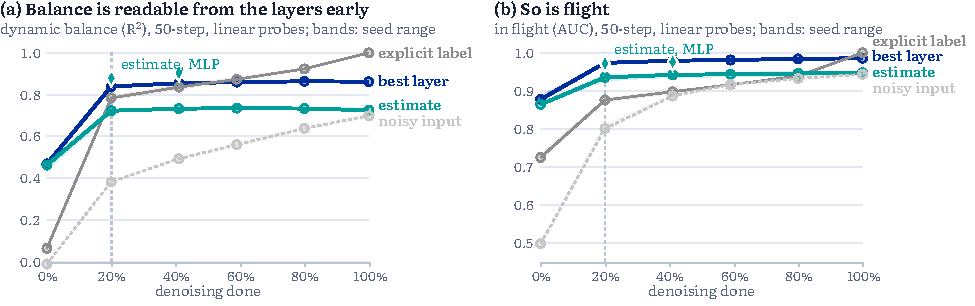
\includegraphics[width=\linewidth]{figures/web/fig_probe_steps.pdf}
\caption{Probe scores across denoising for the 50-step model (lines: mean over three seeds; bands: range). The best layer (deep blue) reads the final motion's dynamic balance and flight early, and so does an MLP reading everything the model's own estimate shows (teal diamonds, measured at 20\% and 40\%; bars: standard deviation). In most figures, teal marks readouts of the estimate, deep blue the model's layers, gray the context, and red the physics of a motion (airborne arcs, floating).}
\label{fig:steps}
\end{figure}

\begin{table}[t]
\centering
\caption{The standard comparison at 20\% of denoising (mean $\pm$ standard deviation over seeds). Best layer: the best of the eight layers per seed, linear probe. Explicit: the label computed from the model's clean-motion estimate. Estimate, linear: a linear probe on the estimate's 263 features. Noisy input: a linear probe on $\vx_t$.}
\label{tab:naive}
\begin{tabular}{llcccc}
\toprule
Model & Target & Best layer & Explicit & Estimate, linear & Noisy input \\
\midrule
\multirow{5}{*}{50-step} & Dynamic balance ($R^2$) & 0.838 $\pm$ 0.001 & 0.783 $\pm$ 0.009 & 0.723 $\pm$ 0.007 & 0.383 $\pm$ 0.006 \\
 & Static balance ($R^2$) & 0.759 $\pm$ 0.014 & 0.769 $\pm$ 0.019 & 0.673 $\pm$ 0.014 & 0.241 $\pm$ 0.007 \\
 & Lowest foot ($R^2$) & 0.868 $\pm$ 0.022 & 0.921 $\pm$ 0.005 & 0.817 $\pm$ 0.029 & 0.396 $\pm$ 0.022 \\
 & In flight (AUC) & 0.973 $\pm$ 0.002 & 0.876 $\pm$ 0.005 & 0.935 $\pm$ 0.008 & 0.801 $\pm$ 0.010 \\
 & Flight gravity ($R^2$) & 0.820 $\pm$ 0.035 & 0.707 $\pm$ 0.079 & 0.547 $\pm$ 0.053 & 0.209 $\pm$ 0.046 \\
\midrule
\multirow{5}{*}{1000-step} & Dynamic balance ($R^2$) & 0.697 $\pm$ 0.029 & 0.655 $\pm$ 0.008 & 0.550 $\pm$ 0.031 & 0.175 $\pm$ 0.003 \\
 & Static balance ($R^2$) & 0.560 $\pm$ 0.058 & 0.546 $\pm$ 0.019 & 0.508 $\pm$ 0.066 & 0.181 $\pm$ 0.009 \\
 & Lowest foot ($R^2$) & 0.804 $\pm$ 0.020 & 0.860 $\pm$ 0.008 & 0.766 $\pm$ 0.012 & 0.303 $\pm$ 0.016 \\
 & In flight (AUC) & 0.926 $\pm$ 0.003 & 0.788 $\pm$ 0.003 & 0.893 $\pm$ 0.001 & 0.759 $\pm$ 0.010 \\
 & Flight gravity ($R^2$) & 0.692 $\pm$ 0.023 & 0.691 $\pm$ 0.060 & 0.405 $\pm$ 0.176 & 0.193 $\pm$ 0.022 \\
\bottomrule
\end{tabular}

\end{table}

Linear probes recover the final motion's physics from the activations well before sampling ends (Figure~\ref{fig:steps}, Table~\ref{tab:naive}). At 20\% of denoising, the best layer of the 50-step model reaches $R^2 = 0.838 \pm 0.001$ for dynamic balance, 0.868 for the lowest-foot height and 0.820 for flight gravity, and an AUC of 0.973 for flight. In these data the flight-gravity score mostly reflects whether an airborne body floats or falls (Section~\ref{sec:fairresults}). Layer 7 is the best layer for dynamic balance in all six runs. The result transfers across prompt types: for dynamic balance at 20\%, the best layer scores 0.835 on curated prompts and 0.839 on test captions. The 1000-step model is less readable at the same fraction of denoising (0.697 for dynamic balance).

Taken at face value, the standard comparison suggests hidden knowledge. For dynamic balance, flight and, on the 50-step model, gravity, the best layer beats both the explicit label and the linear probe on the estimate at the same step. For dynamic balance the gap over the explicit label is $+0.045$ to $+0.065$ in the three 50-step seeds and $+0.018$ to $+0.060$ in the three 1000-step seeds. Only the lowest-foot height, which the estimate shows directly, and static balance on the 50-step model (0.769 against 0.759) favor the explicit label, and flight gravity on the 1000-step model is a tie (0.692 against 0.691).

\subsection{The advantage disappears under a fair readout}
\label{sec:fairresults}

\begin{table}[t]
\centering
\caption{Tuned readouts at 20\% of denoising, seeds pooled, every readout tuned on held-out prompts (Section~\ref{sec:fair}). Pooled $R^2$, or AUC for flight and floats or falls; the best tuned readout in bold. Both: estimate and layer, tuned with fallback. Gain: Both minus Estimate, with 95\% prompt-bootstrap intervals, pooled and within prompt and frame. ``Jump prompts'': the jump-heavy runs. --: too few prompts for an interval. 0 (all folds): the fallback kept the estimate in every fold, so the gain is zero by construction (Table~\ref{tab:gaindetail}).}
\label{tab:tuned}
\resizebox{\linewidth}{!}{\begin{tabular}{llccccccc}
\toprule
& & & & \multicolumn{3}{c}{Tuned on held-out prompts} & \multicolumn{2}{c}{Gain from adding the layer [95\% CI]} \\
\cmidrule(lr){5-7} \cmidrule(lr){8-9}
Target & Model & Explicit & Layer, ridge & Estimate & Layer & Both & Pooled score & Within prompt and frame \\
\midrule
Dynamic balance & 50-step & 0.784 & 0.850 & \textbf{0.889} & 0.863 & \textbf{0.889} & $+0.000$ [$-0.001$, $+0.001$] & $+0.000$ [$-0.001$, $+0.001$] \\
Dynamic balance & 1000-step & 0.655 & 0.720 & \textbf{0.779} & 0.765 & 0.777 & $-0.002$ [$-0.005$, $-0.000$] & $-0.001$ [$-0.003$, $+0.000$] \\
Dynamic balance & MotionDiffuse & 0.124 & 0.620 & \textbf{0.823} & 0.700 & \textbf{0.823} & $0$ (all folds) & $0$ (all folds) \\
\addlinespace[2pt]
Static balance & 50-step & 0.771 & 0.780 & \textbf{0.830} & 0.800 & 0.828 & $-0.001$ [$-0.004$, $+0.002$] & $-0.002$ [$-0.006$, $+0.002$] \\
Static balance & 1000-step & 0.548 & 0.592 & \textbf{0.671} & 0.647 & \textbf{0.671} & $0$ (all folds) & $0$ (all folds) \\
Static balance & MotionDiffuse & 0.103 & 0.537 & \textbf{0.729} & 0.547 & \textbf{0.729} & $0$ (all folds) & $0$ (all folds) \\
\addlinespace[2pt]
In flight & 50-step & 0.876 & 0.977 & \textbf{0.976} & 0.971 & 0.972 & $-0.004$ [$-0.008$, $-0.000$] & $-0.008$ [$-0.014$, $-0.002$] \\
In flight & 1000-step & 0.788 & 0.934 & \textbf{0.935} & 0.932 & \textbf{0.935} & $-0.000$ [$-0.003$, $+0.002$] & $+0.002$ [$-0.000$, $+0.005$] \\
In flight & MotionDiffuse & 0.778 & 0.951 & \textbf{0.943} & 0.905 & 0.939 & $-0.004$ [$-0.009$, $-0.001$] & $-0.001$ [$-0.006$, $+0.003$] \\
In flight & 50-step, jump prompts & 0.926 & 0.981 & \textbf{0.984} & 0.981 & 0.983 & $-0.001$ [$-0.002$, $-0.000$] & $-0.001$ [$-0.002$, $+0.001$] \\
In flight & 1000-step, jump prompts & 0.878 & 0.955 & 0.960 & 0.961 & \textbf{0.962} & $+0.001$ [$-0.000$, $+0.003$] & $+0.001$ [$-0.002$, $+0.003$] \\
In flight & MotionDiffuse, jump prompts & 0.734 & 0.978 & \textbf{0.975} & 0.972 & \textbf{0.975} & $+0.000$ [$-0.001$, $+0.002$] & $+0.002$ [$-0.000$, $+0.004$] \\
\addlinespace[2pt]
Floats or falls & 50-step & 0.931 & 0.990 & 0.980 & \textbf{0.988} & \textbf{0.988} & $+0.008$ [$+0.001$, $+0.015$] & $+0.050$ [$-0.007$, $+0.099$] \\
Floats or falls & 1000-step & 0.922 & 0.980 & 0.964 & \textbf{0.976} & 0.967 & $+0.003$ [$-0.001$, $+0.008$] & $+0.008$ [$-0.013$, $+0.029$] \\
Floats or falls & MotionDiffuse & 0.883 & 0.988 & 0.940 & \textbf{0.988} & 0.966 & $+0.026$ [$+0.007$, $+0.055$] & -- \\
Floats or falls & 50-step, jump prompts & 0.837 & 0.971 & \textbf{0.974} & 0.969 & \textbf{0.974} & $-0.000$ [$-0.009$, $+0.008$] & $-0.000$ [$-0.014$, $+0.016$] \\
Floats or falls & 1000-step, jump prompts & 0.667 & 0.973 & 0.966 & \textbf{0.969} & 0.967 & $+0.001$ [$-0.001$, $+0.003$] & $-0.002$ [$-0.009$, $+0.006$] \\
Floats or falls & MotionDiffuse, jump prompts & 0.741 & 0.836 & 0.827 & 0.784 & \textbf{0.828} & $+0.001$ [$-0.017$, $+0.017$] & $+0.004$ [$-0.018$, $+0.024$] \\
\addlinespace[2pt]
Fall rate (falling only) & 50-step & 0.171 & 0.267 & $-0.168$ & \textbf{0.217} & 0.084 & $+0.253$ [$+0.060$, $+0.505$] & $+0.046$ [$-0.041$, $+0.127$] \\
Fall rate (falling only) & 1000-step & 0.209 & 0.115 & $-0.069$ & \textbf{0.090} & 0.013 & $+0.082$ [$-0.035$, $+0.167$] & $+0.106$ [$+0.020$, $+0.195$] \\
Fall rate (falling only) & 50-step, jump prompts & 0.152 & 0.374 & 0.351 & 0.427 & \textbf{0.428} & $+0.077$ [$+0.051$, $+0.107$] & $+0.073$ [$+0.045$, $+0.098$] \\
Fall rate (falling only) & 1000-step, jump prompts & 0.161 & 0.273 & 0.287 & 0.309 & \textbf{0.363} & $+0.076$ [$+0.053$, $+0.096$] & $+0.021$ [$+0.006$, $+0.037$] \\
Fall rate (falling only) & MotionDiffuse, jump prompts & 0.289 & 0.326 & 0.365 & 0.326 & \textbf{0.390} & $+0.025$ [$+0.003$, $+0.047$] & $+0.017$ [$-0.001$, $+0.036$] \\
\bottomrule
\end{tabular}
}
\end{table}

\begin{figure}[t]
\centering
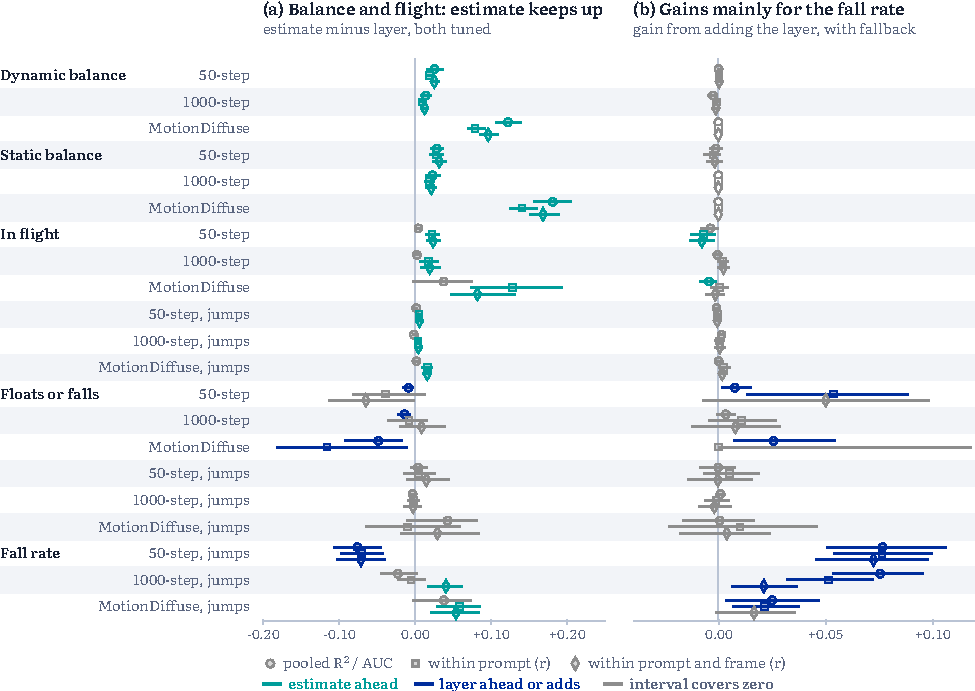
\includegraphics[width=\linewidth]{figures/web/fig_gain.pdf}
\caption{The fair comparison (tuned readouts, seeds pooled, 95\% prompt-bootstrap intervals). (a)~Tuned estimate minus tuned layer: positive favors the estimate. (b)~The gain from adding the layer to the estimate, with fallback. Marker shape gives the score; color gives the verdict: teal where the estimate is ahead, deep blue where the layer is ahead or adds, gray where the interval covers zero, and open markers at zero where the fallback kept the estimate in every fold. In (b), clear gains appear only for the fall rate on the jump prompts (``jumps'') and for floating in the small main data sets; balance and flight show none. Not drawn: scores without an interval (too few prompts) and the main data's fall rate (1,147 and 1,620 falling frames, intervals up to about $\pm 0.25$; Table~\ref{tab:tuned}).}
\label{fig:gain}
\end{figure}

Table~\ref{tab:tuned} and Figure~\ref{fig:gain} compare the readouts with the three seeds of each model pooled and every readout tuned on held-out prompts (Section~\ref{sec:fair}). A first version with one fixed MLP per seed gives the same ordering (Appendix~\ref{app:fixedmlp}). For balance and flight the estimate is read as well as the layer: for both balance measures its tuned readout beats the tuned layer, by 0.015 to 0.029 in $R^2$ on both MDM checkpoints and by 0.12 and 0.18 on MotionDiffuse, and for flight the estimate ties or leads. Adding the layer to the estimate gains nothing. With the readout that may fall back to the estimate, every interval covers zero or lies below it, across prompts and within prompt and frame, and so does every interval in two refits with other validation splits and initializations, run for dynamic balance on the 50-step model. The layer sweep shows the same for every layer: none adds more than 0.007, and only one interval, for flight at layer~7 of the 1000-step model, barely excludes zero (Figure~\ref{fig:layers}). On MDM, whose conditional estimate is a fixed linear map of layer~7, a gain from that layer could come only from directions the output head discards.

This null result is not produced by the estimator. Without the fallback, the larger readout scores within 0.003 of the estimate or below it for balance and flight, so the fallback hides no gain there. It keeps the estimate alone in one to five of the five folds (Table~\ref{tab:gaindetail}). On the scale of Proposition~\ref{prop:vinfo}, the largest balance gain is 0.001 nats, against 0.063 for the fall rate below.

A positive control shows what the protocol can detect (Table~\ref{tab:control}). We take the estimate readout's out-of-fold residual, add noise so that its best linear use would raise $R^2$ by 0.005, 0.01 or 0.02 on the squared-error scale, add it to the layer's activations along a random direction, and rerun the protocol unchanged on the 50-step model. For dynamic balance even the smallest signal is found: the gain is $+0.013$ [$0.009$, $0.017$], more than the linear amount because the tuned readouts extract more, against $+0.000$ [$-0.001$, $0.001$] for the real layer. For flight and floating the pooled AUC, near 0.97, barely moves even at 0.02, partly because the readouts are selected by squared error. The within-prompt-and-frame score does find the signal, from 0.005 for flight and from 0.01 for floating on the jump prompts, and on that score the real layer adds nothing ($-0.008$ and $0.000$). For these two targets the evidence for no gain is therefore that score, and a gain below 0.01 for floating could go undetected.

Two details show where the estimate's advantage comes from. First, the readout family matters: restricted to linear readouts, the layer does add a little (up to 0.02 on MDM, 0.05 to 0.07 on MotionDiffuse), so part of what the estimate shows needs a nonlinear readout. Second, on MDM the input matters more than the family: from its 263 raw features alone the tuned estimate only ties the tuned layer, and the physics labels computed from it add about 0.02 for dynamic balance (Table~\ref{tab:raw}). On MotionDiffuse the raw features alone already beat the tuned layer, by 0.12 and 0.18 (Table~\ref{tab:tuned}), and the labels add nothing. A temporal readout that sees all 30 recorded frames gives the same ordering in all six runs (Appendix~\ref{app:impl}). In the terms of Section~\ref{sec:fair}, the usable information the layer adds about balance and flight depends on the readout family, and for the most flexible readouts we tried it is indistinguishable from zero.

\begin{figure}[t]
\centering
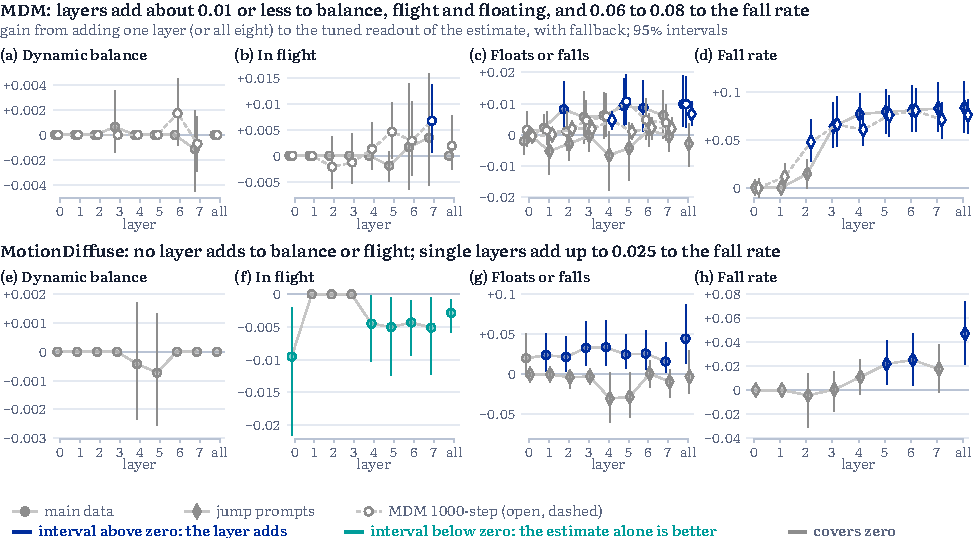
\includegraphics[width=\linewidth]{figures/web/fig_layers.pdf}
\caption{The gain from adding one layer, or all eight, to the tuned readout of the estimate (with fallback, 20\% of denoising, 95\% intervals; colors as in Figure~\ref{fig:gain}). Circles: main data; diamonds: jump prompts; open markers and dashed lines: the 1000-step model. Top row, MDM: only the fall rate rises well above zero, from layer~3 on (layer~2 on the 1000-step model); the floating gains stay at about 0.01 or less. Bottom row, MotionDiffuse: the same pattern with a smaller fall-rate gain, from layers 5 to 7, and a floating gain only on the main data's 50 prompts. The main data's fall rate is not shown (too few falling frames).}
\label{fig:layers}
\end{figure}

\paragraph{Flight gravity: floating and falling.} The fitted flight gravity mixes two questions. In the main data most of its labelled frames (76\% and 83\%) lie in floating stretches, so its score mostly measures whether an airborne body floats or falls, and only 57 and 78 prompts contain falling frames, too few for reliable tuned readouts. We therefore split the target (Section~\ref{sec:labels}) and use the jump-heavy runs, in which most labelled frames fall (11,640 and 13,444 frames from 233 and 240 prompts).

Whether an airborne body floats or falls is visible in the estimate on the jump prompts, where 236 prompts have airborne stretches on the 50-step model. Its tuned readout reaches an AUC of 0.97 on both MDM checkpoints, and no single layer, nor all eight together, adds more than 0.007 in pooled AUC (Figure~\ref{fig:layers}). Across the three fits the layer adds at most $0.004$ in pooled AUC, and $0.019$ [$0.008$, $0.030$] within prompt in one of them. The layer adds more only in the smaller main data, where just 106 prompts have airborne stretches. There, on the 50-step model, it adds $+0.008$ [$0.001$, $0.015$] in pooled AUC and $+0.054$ [$0.013$, $0.089$] in the within-prompt correlation, and in two refits up to $0.014$ pooled and $0.08$ to $0.11$ within prompt and frame.

\begin{figure}[t]
\centering
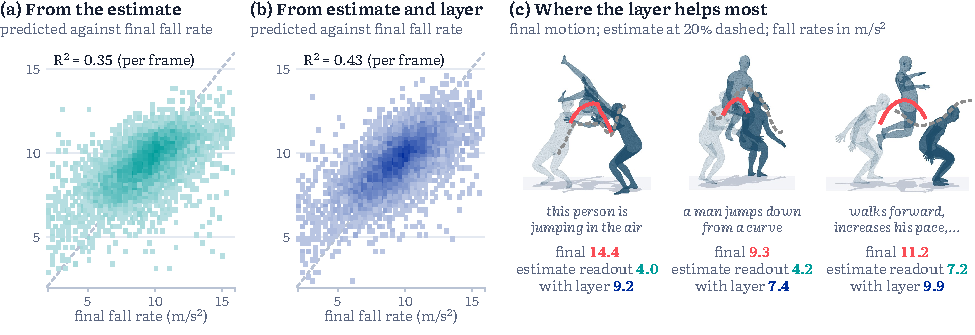
\includegraphics[width=\linewidth]{figures/web/fig_layer_knows.pdf}
\caption{Held-out predictions of the final fall rate on the jump prompts (50-step model, 20\% of denoising, tuned readouts; density of falling stretches in cells of 0.25\,m/s$^2$, darker for more). (a)~From the estimate alone and (b)~with layer~5 added (with fallback); dashed: perfect prediction; $R^2$ per frame, as in Table~\ref{tab:tuned}. (c)~Among jumps that travel at least 0.4\,m, the three where adding the layer reduces the error most, selected for that reason: the final motion at take-off, apex and landing, its center-of-mass path (red while airborne), and the estimate's path at 20\% (dashed).}
\label{fig:layerknows}
\end{figure}

\begin{figure}[t]
\centering
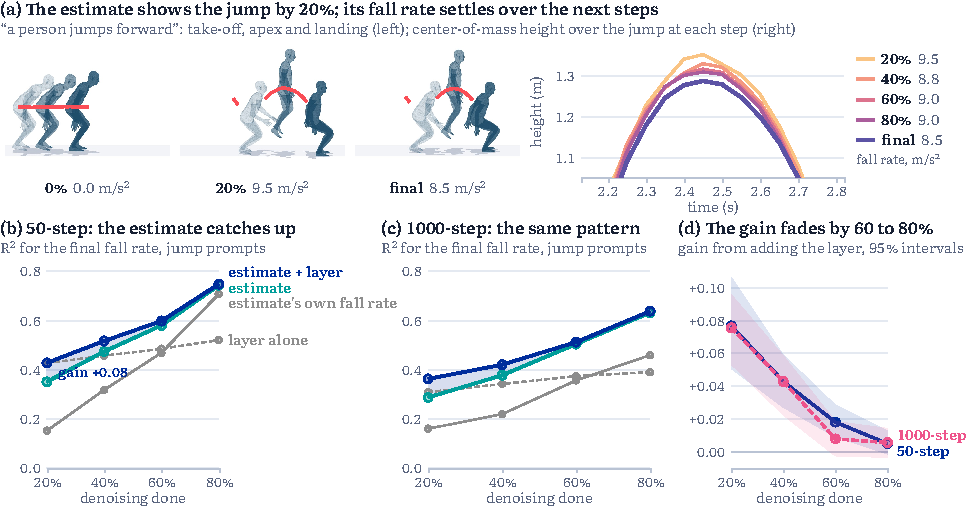
\includegraphics[width=\linewidth]{figures/web/fig_steps_fall.pdf}
\caption{The fall rate of jumps across denoising (jump prompts, layer~5, tuned readouts, seeds pooled). (a)~A typical jump, drawn from the estimate at 0\% and 20\% of denoising and from the final motion (center of mass red while airborne), and its center-of-mass height at every recorded step with that step's fitted fall rate. At 0\% the estimate is a crouched average pose; from 20\% the jump is in place, and its height and fall rate change by only a few centimeters and about 1\,m/s$^2$ afterwards. The jump is chosen by a fixed rule: among falling stretches of the 50-step runs that travel at least 0.4\,m, the one whose 20\% fall-rate error is the median (1.0\,m/s$^2$). (b, c)~$R^2$ for the final fall rate from the estimate and from estimate and layer together; the shaded gap is the gain. Gray: the estimate's own fitted fall rate, and the layer alone. (d)~The gain, with 95\% intervals: largest at 20\%, below 0.02 by 60\%.}
\label{fig:stepsfall}
\end{figure}

The fall rate of the stretches that do fall is the one case in which the layers know more. On the jump prompts of the 50-step model, adding the layer raises $R^2$ from 0.35 to 0.43, a gain of $+0.077$ [$0.051$, $0.107$], or 0.063 nats (Tables~\ref{tab:tuned} and~\ref{tab:gaindetail}, Figure~\ref{fig:layerknows}), with similar gains within prompt and frame and in two refits. With more training prompts the gain first shrinks and then levels off from 100 prompts on (0.085, then 0.077; Figure~\ref{fig:tunedcurve}b). It replicates on the 1000-step model ($+0.076$ [$0.053$, $0.096$]), though there it is smaller within prompt and frame ($+0.021$) and with fewer training prompts (Figure~\ref{fig:tunedcurve}c), and the layer alone is no longer clearly ahead of the estimate (0.309 against 0.287, an interval that covers zero), so the two carry partly different information. On both MDM checkpoints every layer from 3 to 7 adds 0.06 to 0.08 (Figure~\ref{fig:layers}). The standard comparison overstates even this genuine case: the layer's ridge probe beats the explicit label by three times the conditional gain on the 50-step model and 1.5 times on the 1000-step model, because the fall rate fitted to a 20\% estimate predicts the final one poorly.

Four checks leave the gain in place. It is not only the layer knowing where a jump is: in 92\% of the 11,640 falling frames, from 7,125 falling stretches, the 20\% estimate is airborne too, and there the layer still adds $+0.069$. It is not a weak readout of the estimate's timing: the estimate's readout already includes its own fitted fall rate, and a temporal readout over all 30 recorded frames still leaves the layer ahead in every seed (Appendix~\ref{app:impl}). It is not the text: giving the readout the prompt's CLIP embedding, the model's own text input, does not help on held-out prompts, and the layer's gain beyond estimate and text is unchanged. And label noise is not the ceiling: on real motion capture the gravity label's spread would allow an $R^2$ of 0.81 to 0.91 (Appendix~\ref{app:realmotion}).

The gain is, however, transient (Figure~\ref{fig:stepsfall}). At 40\% of denoising layer~5 still adds 0.043 on both MDM checkpoints (Figure~\ref{fig:stepsfall}d). By 60\% no layer adds more than 0.02, and at 80\% the interval for layer~5 covers zero, because the estimate's readout improves faster than the layer's. A separate layer sweep gives up to about 0.06 at 40\%, and the same readout differs by up to 0.016 between that sweep and the step run. At a fifth of the denoising steps, then, MDM's middle and late layers carry information about how fast a jump will fall that its estimate does not yet show in any form we could read: a step-wise case of a model knowing more than it shows, of the kind the video studies report. Such a gain must vanish by the end of sampling, when the final motion is a function of the estimate, so what the measurement adds is its size and duration: about 0.08 in $R^2$, for about two fifths of the trajectory.

\paragraph{A second model.} MotionDiffuse (Section~\ref{sec:models}) predicts the noise, receives the text in every layer and uses no guidance, and it gives the same picture for balance and flight. On its main data the tuned estimate beats the tuned layer by 0.12 in $R^2$ for dynamic balance and 0.18 for static balance, more than on MDM. Adding any one of its eight layers gains at most 0.001 for dynamic balance, and its chosen layers add nothing for static balance or flight. Floating follows MDM's pattern: on the main data, where only 50 prompts have airborne stretches, its layers add 0.016 to 0.034 in AUC and the layer alone beats the estimate (0.988 against 0.940), while on its jump prompts (2,940 motions, 235 prompts with such stretches) they add nothing, and the same holds for flight and for the unsplit flight gravity (at most $+0.002$).

The fall rate again shows a gain, but a smaller and less stable one. At 20\% of denoising (step 200 of 1000), adding layer~6 raises $R^2$ from 0.365 to 0.390, $+0.025$ [$0.003$, $0.047$] (Table~\ref{tab:tuned}, Figures~\ref{fig:gain} and \ref{fig:layers}). It holds within prompt ($+0.022$ [$0.007$, $0.038$]), but within prompt and frame its interval covers zero ($+0.017$ [$-0.001$, $0.036$]), and in two refits with other validation splits and initializations it is $+0.022$ [$0.007$, $0.041$] and 0, the fallback keeping the estimate in every fold of the second. It again comes from the later layers (layers 5 to 7 add 0.018 to 0.025 and all eight together 0.047, layers 0 to 3 nothing), the text does not explain it (estimate, text and layer together gain the same $+0.025$ over the estimate as without the text), and it fades with denoising: $+0.012$ [$0.003$, $0.022$] at 40\% and $+0.007$ [$-0.002$, $0.016$] at 60\%.

At matched noise the gap to MDM is larger still, because the same fraction of denoising is not the same noise level on the two models. At 20\% MotionDiffuse's signal-to-noise ratio is 0.002, against MDM's 0.10, and it reaches MDM's range only between 40 and 60\% (Table~\ref{tab:snr}). At 60\%, with a ratio of 0.24, between MDM's at 20\% (0.10) and 40\% (0.52), MotionDiffuse's gain is $+0.007$, against MDM's $+0.077$ and $+0.043$ at those steps.

Across targets and on all three models, then, a readout of what the model shows, tuned as carefully as the probe on its activations, accounts for what the activations predict about the final motion's balance and flight, and about floating on the jump prompts. In the smaller main data sets adding a layer does help with floating (the chosen layer gains up to 0.026 in AUC, removing up to 43\% of the misranked pairs, and single MotionDiffuse layers up to 0.034; Table~\ref{tab:gaindetail}). The apparent knowledge in Table~\ref{tab:naive} came from comparing a trained probe on the activations with an untrained or linear readout of the estimate. The fall rate of jumps is the exception, and it is found by the same controls that remove the other advantages.

\subsection{Small training sets can reverse the comparison}
\label{sec:learning}

\begin{figure}[t]
\centering
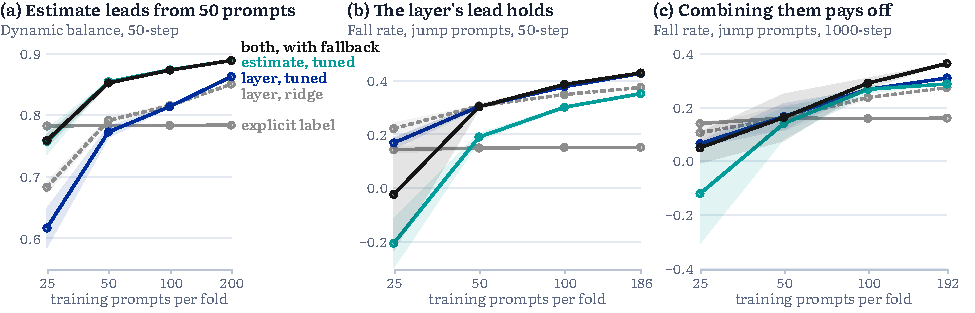
\includegraphics[width=\linewidth]{figures/web/fig_tuned_curve.pdf}
\caption{Tuned readouts trained on fewer prompts (seeds pooled, same test folds; two draws per size below the full set; lines: mean, bands: range). (a)~Dynamic balance: the explicit label wins at 25 prompts, and from 50 on the estimate leads the layer. (b)~The fall rate of jumps, 50-step model: the layer leads at every size. (c)~The same target, 1000-step model: the gain from combining estimate and layer grows from 0.02 to 0.08 only with the full training set.}
\label{fig:tunedcurve}
\end{figure}

The pilot study pointed the other way: with 64 prompts and one held-out set of 12, the explicit label beat the best layer on dynamic balance (0.832 against 0.814). Training size explains it: the one-feature explicit label barely depends on the number of training prompts, while the 512-feature linear layer probe overtakes it only between 52 and 100 training prompts (Appendix~\ref{app:fixedmlp}, Figure~\ref{fig:learning}), and the pilot's 12-prompt test set was also too small to fix the sign. Tuned readouts with pooled seeds show the same dependence (Figure~\ref{fig:tunedcurve}). For dynamic balance, the one-feature explicit label still beats every trained readout at 25 training prompts on the 50-step model (0.783, against 0.757 for the tuned estimate and 0.617 for the tuned layer), and from 50 prompts on the tuned estimate leads the tuned layer at every size (0.854 against 0.773 at 50, 0.889 against 0.863 at 200). The lead narrows as data grows, from 0.060 at 100 prompts to 0.026 at 200 (0.026 to 0.015 on the 1000-step model), so with much larger training sets the layer's readout could catch up. The gain from adding the layer, which is what bears on hidden knowledge, stays at zero at every size we measured ($-0.003$ to $+0.003$ with the fallback readout). For the fall rate of jumps on the 50-step model the layer leads at every size, and its lead over the estimate stops shrinking: 0.113 at 50 prompts, 0.076 at 100 and 0.075 at 186. On the 1000-step model the layer alone leads by at most 0.026 from 50 prompts on, and the gain from adding it to the estimate is 0.022 and 0.023 at 50 and 100 prompts and 0.076 at 192. A comparison at one training size can favor either side, and only a lead that persists as data grows is evidence about the model. Video probing benchmarks are of a similar size: the IntPhys development set used in Section~\ref{sec:video} has 360 videos.

\subsection{Early warning: the estimate is enough, and the payoff is small}
\label{sec:early}

\begin{table}[t]
\centering
\begin{minipage}[t]{0.37\linewidth}
\centering
\caption{The training-free rule ``abort if the decoded estimate shows any floating''. Precision: flagged samples that do float. Recall: floating samples flagged.}
\label{tab:detector}
\resizebox{\linewidth}{!}{\begin{tabular}{llccc}
\toprule
Model & Check at & Flagged & Precision & Recall \\
\midrule
50-step & 20\% & 7.0\% & 80\% & 59\% \\
50-step & 40\% & 7.0\% & 88\% & 65\% \\
1000-step & 20\% & 10.1\% & 82\% & 47\% \\
1000-step & 40\% & 11.1\% & 84\% & 52\% \\
\bottomrule
\end{tabular}
}
\end{minipage}\hfill
\begin{minipage}[t]{0.6\linewidth}
\centering
\caption{Compute saved by aborting at 20\% of denoising, with the final check kept, against finish-then-filter at the same delivered failure (its budget of 2, 3 or 5 tries). The trained readouts (ridge on frame-averaged inputs: everything the estimate shows, one layer, or both) abort the same share of samples as the rule.}
\label{tab:savings}
\resizebox{\linewidth}{!}{\begin{tabular}{lccccccc}
\toprule
Model & Delivered & Finish, then filter & \multicolumn{5}{c}{Compute saved by early abort} \\
\cmidrule(lr){4-8} & floating & (compute) & estimate rule & estimate readout & layer probe & readout + layer & perfect detector \\
\midrule
50-step & 3.8\% & 1.24 & 6.7\% & 6.8\% & 4.5\% & 4.5\% & 14.9\% \\
50-step & 4.5\% & 1.15 & 4.8\% & 5.1\% & 5.1\% & 5.5\% & 10.2\% \\
50-step & 5.5\% & 1.09 & 3.4\% & 3.6\% & 3.6\% & 3.8\% & 6.7\% \\
1000-step & 4.6\% & 1.39 & 9.9\% & 9.8\% & 10.7\% & 10.2\% & 22.5\% \\
1000-step & 6.8\% & 1.27 & 6.9\% & 6.9\% & 6.8\% & 6.5\% & 17.0\% \\
1000-step & 9.4\% & 1.18 & 4.3\% & 4.4\% & 4.0\% & 3.7\% & 11.9\% \\
\bottomrule
\end{tabular}
}
\end{minipage}
\end{table}

\begin{figure}[t]
\centering
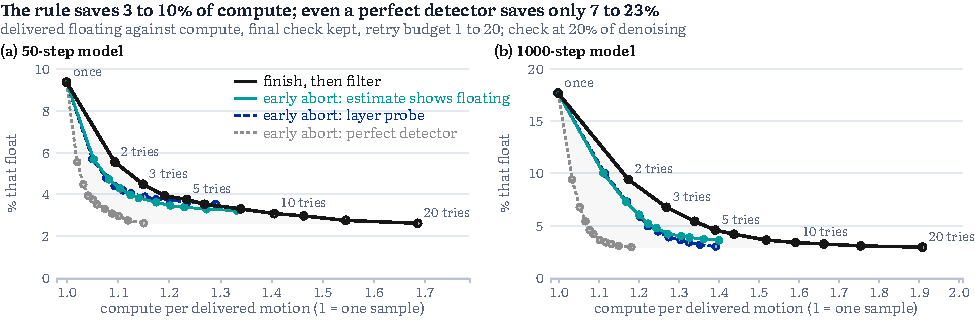
\includegraphics[width=\linewidth]{figures/web/fig_early.pdf}
\caption{Delivered floating against compute, with the final check kept and the retry budget varied from 1 to 20 tries (labels on the finish-then-filter curve). Aborting at 20\% of denoising when the decoded estimate shows floating (teal) moves the curve only slightly, and a layer probe (deep blue) moves it about as much. The shaded region between finish-then-filter and a perfect detector bounds what any early signal could save.}
\label{fig:early}
\end{figure}

An early signal is useful in practice if it stops samples that will fail. For MDM, the model's own estimate provides one without any training (Table~\ref{tab:detector}). If the estimate shows floating at 20\% of denoising, the final motion floats in 80\% (50-step) and 82\% (1000-step) of cases, and the rule catches 59\% and 47\% of all floating samples. At 40\%, precision rises to 88\% and 84\%. As a per-sample score, the estimate's own floating rate also ranks samples within a prompt better than trained readouts. At 20\%, its Spearman correlation with the final floating rate after removing prompt means is 0.57 (50-step) and 0.46 (1000-step), against 0.34 and 0.33 for a ridge readout of everything the estimate shows, 0.26 and 0.28 for the same ridge on a layer, and 0.29 and 0.28 for the two together: at the sample level, too, the layer adds nothing to the estimate's readout, at least for these ridge readouts of frame-averaged inputs. The prompt's text embedding alone predicts the floating rate only weakly on held-out prompts (Spearman 0.25 and 0.23).

The compute payoff is small (Table~\ref{tab:savings}, Figure~\ref{fig:early}). Checking the final motion costs almost nothing, so finish-then-filter is the baseline to beat: with two tries it delivers 5.5\% floating motions at 1.09 times the compute of a single sample (50-step), and 9.4\% at 1.18 (1000-step), against 9.4\% and 17.7\% when generating once. Early abort without the final check bottoms out at 6.6 to 6.9\% and 13.6 to 14.5\% floating with the training-free rule, and at 5.5 to 6.3\% and 10.3 to 12.0\% with the trained readouts. Without the final check, the rule at 20\% of denoising delivers within 0.9 percentage points of finish-then-filter at the same compute (mixing budgets of one and two tries), and at 40\% it falls behind. With the final check kept, aborting at 20\% with the rule saves 3.4 to 6.7\% of compute at matched failure for the 50-step model and 4.3 to 9.9\% for the 1000-step model, more at stricter targets. The trained readouts, set to abort the same share of samples, save about as much (3.6 to 10.7\%) with no consistent order between them: the readout of the estimate, the layer probe, and the two together. At the strictest 50-step target the two that use the layer save less (4.5\%, against 6.7 to 6.8\%). Random aborts give no gain. Even a perfect detector would save only 6.7 to 14.9\% and 11.9 to 22.5\%. This ceiling has a closed form.
\begin{proposition}\label{prop:ceiling}
Let prompt $u$ fail in a share $p_u$ of its samples, let an attempt aborted early cost a fraction $\tau$ of a full sample, and compare strategies at the same retry budget $B$ with the final check kept, prompts weighted equally. A perfect detector saves the fraction
\begin{equation}
    S_B \;=\; (1-\tau)\, \frac{\sum_u \sum_{j=1}^{B-1} p_u^{\,j}}{\sum_u \sum_{j=0}^{B-1} p_u^{\,j}}
\end{equation}
of the compute of finish-then-filter at the same delivered failure: $1-\tau$ times the share of finish-then-filter's attempts that are discarded. At every budget, no other detector that checks at the same step uses less compute or delivers fewer failures.
\end{proposition}
With the measured $p_u$ and $\tau = 0.22$ (50-step) and $0.201$ (1000-step), the formula gives 0.067, 0.101 and 0.148 at budgets 2, 3 and 5 for the 50-step model, and 0.120, 0.172 and 0.226 for the 1000-step model, within 0.0015 of the simulation (proof in Appendix~\ref{app:proofs}). The ceiling is low because floating affects only 9 to 18\% of samples and concentrates in particular prompts: after 20 tries, 2.6 to 3.7\% of delivered motions still float, from prompts such as walking on a balance beam that float in nearly every sample.

\subsection{A related readout issue in a video diffusion model}
\label{sec:video}

\begin{table}[t]
\centering
\caption{IntPhys development set, plausibility read from the clean Wan~2.1 VAE latent (360 videos, 90 scenarios; scenario-grouped 5-fold cross-validation, 10 repeats, 3 for the nonlinear temporal probe; mean $\pm$ standard deviation). Pairwise: share of possible/impossible pairs within a scenario in which the possible video scores higher. Chance is 50\% for both.}
\label{tab:intphys}
\begin{tabular}{lcc}
\toprule
Readout of the clean VAE latent & Per-video (\%) & Pairwise (\%) \\
\midrule
\multicolumn{3}{l}{\emph{Linear in the latent}} \\
\quad Pooled over time and space & 50.1 $\pm$ 0.5 & 52.1 $\pm$ 1.5 \\
\quad Time kept & 51.5 $\pm$ 0.7 & 50.4 $\pm$ 1.3 \\
\quad Time + $4{\times}4$ space & 50.9 $\pm$ 1.1 & 54.4 $\pm$ 1.2 \\
\quad Time + $4{\times}4$ space + signed changes & 52.8 $\pm$ 1.1 & 52.2 $\pm$ 2.2 \\
\multicolumn{3}{l}{\emph{Linear after a fixed nonlinearity: absolute frame-to-frame change}} \\
\quad Time kept + $|\Delta|$ & 53.4 $\pm$ 1.2 & 57.4 $\pm$ 2.2 \\
\quad $4{\times}4$ space, $|\Delta|$ only & 61.8 $\pm$ 0.6 & 77.9 $\pm$ 1.7 \\
\quad Time + $4{\times}4$ space + $|\Delta|$ & 62.1 $\pm$ 0.9 & 79.6 $\pm$ 2.3 \\
\multicolumn{3}{l}{\emph{Trained nonlinear readout}} \\
\quad Small temporal CNN & 50.4 $\pm$ 0.3 & 53.9 $\pm$ 2.5 \\
\midrule
Shuffled labels (1,000 shuffles, last $|\Delta|$ row; mean, 95th pct.) & 50.1, 53.1 & 49.9, 56.7 \\
\bottomrule
\end{tabular}

\end{table}

\citet{esmati2026invisible} decode plausibility linearly from the transformer states of video diffusion models, including the 1.3B Wan model \citep{wan2025}, find the clean VAE latent at chance, and conclude that the diffusion model constructs the signal (Section~\ref{sec:related}). Their transformer probes act on states averaged over all tokens. Their public code does not include the latent baseline, so we reproduce it by averaging the latent in the same way. We encode the IntPhys development set \citep{riochet2018intphys} with the Wan~2.1 VAE at the resolution of their IntPhys setting ($256 \times 256$; 97 frames, giving a latent of 16 channels by 25 frames by $32 \times 32$) and read plausibility with ridge classifiers, keeping the four versions of each scenario on the same side of every split (Appendix~\ref{app:video}).

The fully averaged latent is at chance, as they report (Table~\ref{tab:intphys}), and so is every readout that is linear in the latent: keeping the time axis, alone or with a coarse $4 \times 4$ spatial grid, and adding signed frame-to-frame differences, which are themselves linear in the latent, all stay between 50 and 55\% pairwise. One fixed nonlinearity changes this. The absolute frame-to-frame change of the $4 \times 4$ grid features, read linearly, reaches 77.9\% pairwise accuracy on its own, and 79.6\% pairwise and 62.1\% per-video together with the grid features. That readout scores 79 to 82\% pairwise in each of the three IntPhys blocks, and it or the grid's absolute change alone is the best of the readouts we tried in each (Appendix~\ref{app:video} lists them all), so choosing it on any one block and testing on the other two gives the same result. It also beats a label-shuffled null (mean 49.9\%, 95th percentile 56.7\%) in all 1,000 shuffles ($p = 0.001$), and the signed changes do not ($p = 0.31$ pairwise, $0.06$ per video). Without the spatial grid the same transform reaches only 57.4\%. The signal is not a global artifact of how the impossible videos are spliced together: the mean frame-to-frame change is only 1.00 to 1.03 times larger in impossible videos at every step, and training-free ``largest change'' scores, over the whole frame or over any cell of the $4 \times 4$ grid, are at chance (50.0\% pairwise). The readout uses localized changes, consistent with the impossible event itself, an object vanishing, appearing or changing in one region. A small temporal CNN did not train on about 290 training videos.

The averaged baseline in particular has a structural blind spot.
\begin{remark}\label{rem:average}
A linear readout of the time-averaged latent, $w^\top \bar\vz$ with $\bar\vz = \frac1T \sum_t \vz_t$, depends on a video only through $\bar\vz$. It cannot separate videos whose frames differ by a rearrangement in time, or by any change that leaves the average unchanged.
\end{remark}
Impossible events such as a vanishing or teleporting object are mostly changes over time, which an average over all frames largely removes, so chance accuracy of this baseline is no evidence that the latent lacks the signal. The remark does not explain why linear readouts that keep the time axis fail too. The magnitude of change, which they cannot form, is what separates the videos here. Plausibility is therefore not linearly decodable from the clean latent, in agreement with their baseline, but it is present there, and a fixed, training-free transform exposes it. Kinematic statistics of frame-to-frame change likewise detect physics violations in the features of frozen image encoders, where a linear probe on the same features reaches 55.5\% on IntPhys~2 \citep{interno2026geophys}; here the same idea applies to a generator's own VAE latent. By the argument of Section~\ref{sec:fair}, no transformer layer can carry more information about it than this latent together with the text prompt. A transformer that makes the signal linearly decodable has made it more usable, as a good representation should. That alone does not show that the model constructs knowledge absent from its input. Our test does not show that the transformer adds nothing: its per-video accuracy may well exceed our 62\% (they report 81.27\% per-video for the 1.3B Wan model, averaged over transformer blocks and over the categories of IntPhys and a second benchmark, InfLevel).
